\chapter{Una torre más o menos medieval -- II}

\section{Los primeros \emph{bugs} de Cecilia}
\label{sec:primer-bug}

\lettrine[ante=\raisebox{-1.5ex}{\Large ---},lines=2]{H}{ay un
  pequeño} detalle; mirá el piso bien desde arriba ---ad\-vir\-tió
Antonia.

\begin{figure}[ht]
    \centering
    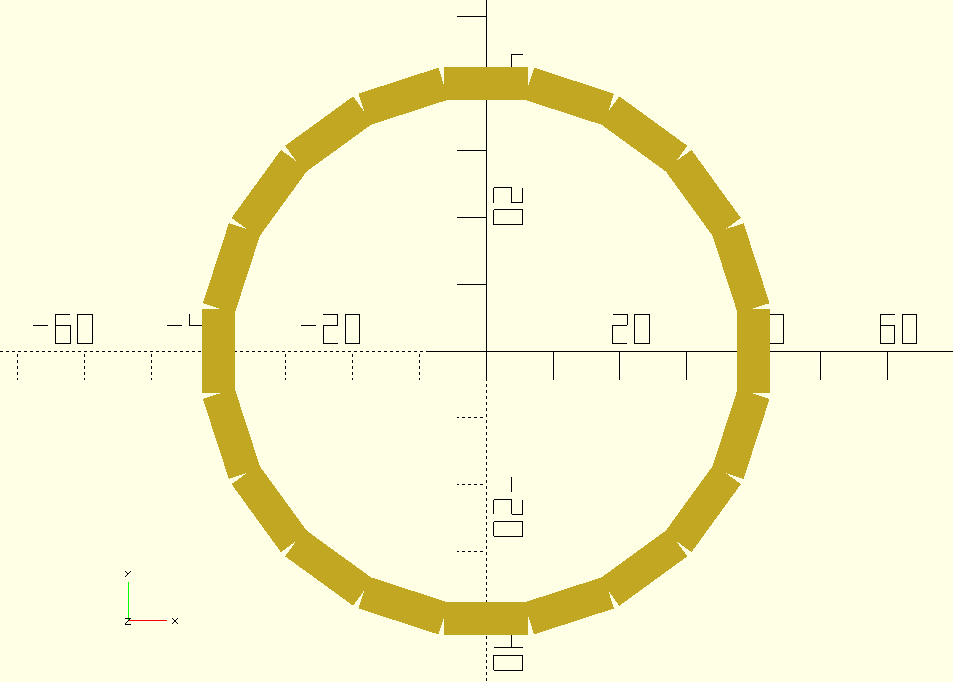
\includegraphics[width=.6\textwidth]{imagenes/piso-cenit}
    \caption{Antonia muestra el piso de ladrillos cenitalmente, a fin
      de que Cecilia detecte un \emph{bug} sutil.}
    \label{fig:piso-cenit}
  \end{figure}


  Cecilia seguía viéndolo hermoso.

  ---A ver, ¿qué me decís del radio?  ¿Es de 40? ---señaló
  Antonia con aire cómplice.

  ---¡Uy!  ¡Tenés razón!  ---Cecilia concedió---. Me quedó un poco más
  grande... ¿Por qué será?

  ---Ah, no sé ---Antonia puso cara de exagerada per\-ple\-ji\-dad---;
  el piso lo escribiste vos. Vos sabrás...

  Cecilia aceptó el reto con una sonrisa. Para apreciar mejor el
  problema, hizo descender el piso por debajo de los ejes de
  coordenadas:

\begin{figure}[ht]
  \begin{minipage}[]{.5\textwidth}
    \begin{lstlisting}
translate([0,0,-20])
  piso(40,5,5,20);
    \end{lstlisting}
  \end{minipage}\hfill
  \begin{minipage}[]{.5\textwidth}
      \centering
      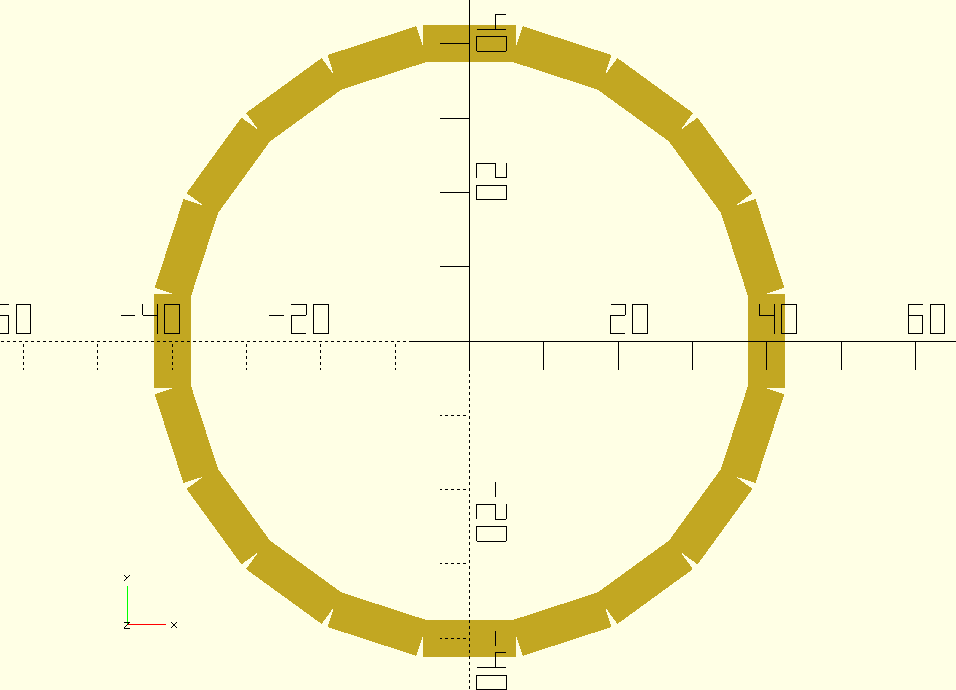
\includegraphics[width=\textwidth]{imagenes/piso-cenit-2}
    \end{minipage}
    \caption{Cecilia desciende el piso a fin de encontrar su
      \emph{bug} poniendo de manifiesto los ejes coordenados.}
  \label{fig:piso-cenit-2}
\end{figure}


<<Hmmm... La marca de los `40' cae justo en el centro de un ladrillo>>
---pensó---. <<Y, sin embargo, a cada uno lo desplacé exactamente 40mm
con la instrucción \lstinline!translate([radio, 0, 0])!... ¿Por qué no
me queda el piso con un radio de 40mm?>>

  Cecilia estaba desorientada. Decidió volver a recorrer todo su
  texto, hasta que sus ojos se detuvieron en la definición del módulo
  \texttt{ladrillo}.

  ---¡Claro! ---dijo, ahora en voz alta, para compartirlo con
  An\-to\-nia---. Si el ladrillo lo hago aparecer centrado, cuando lo
  traslado es su \emph{centro} el que se aleja 40mm.

\begin{figure}[ht]
  \begin{minipage}[]{.5\textwidth}
    \begin{lstlisting}
translate([0,0,-10])
  ladrillo([5,15,5]);
translate([40,0,-10])
  ladrillo([5,15,5]);
    \end{lstlisting}
  \end{minipage}\hfill
  \begin{minipage}[]{.5\textwidth}
      \centering
      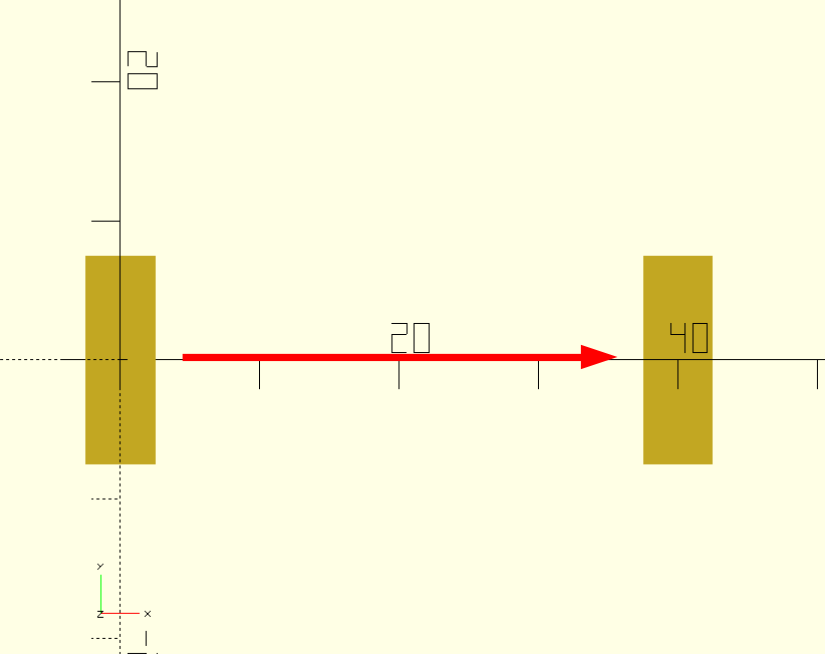
\includegraphics[width=.8\textwidth]{imagenes/ladrillos-bug}
    \end{minipage}
    \caption{Cecilia descubre la razón de su \emph{bug}.}
  \label{fig:ladrillos-bug}
\end{figure}


---Perfecto ---aprobó Antonia---; ahora, ¡a corregirlo!

A Cecilia no le pareció muy difícil lograrlo, una vez que localizó el
problema: se trataba de desplazar el ladrillo una distancia igual al
radio del piso \emph{menos} la mitad del espesor de su pared, lo cual
se conseguía modificando la línea 10:

\begin{lstlisting}
module piso(
 radio,
 altura,
 espesor,
 n_ladrillos) {
  i_alfa=360/n_ladrillos;
  largo=2*PI*radio/n_ladrillos; 
  for (alfa=[0:i_alfa:359])
   rotate([0,0,alfa])
    translate([radio-espesor/2,0,0])
     ladrillo([espesor,largo,altura]); 
}
translate([0,0,-20])
  piso(40,5,5,20);
\end{lstlisting}


\begin{figure}[ht]
%  \centerfloat
  \subbottom[El piso parcialmente resuelto... \vspace{1em} \phantom{a
    la la la la la akldj }]
  {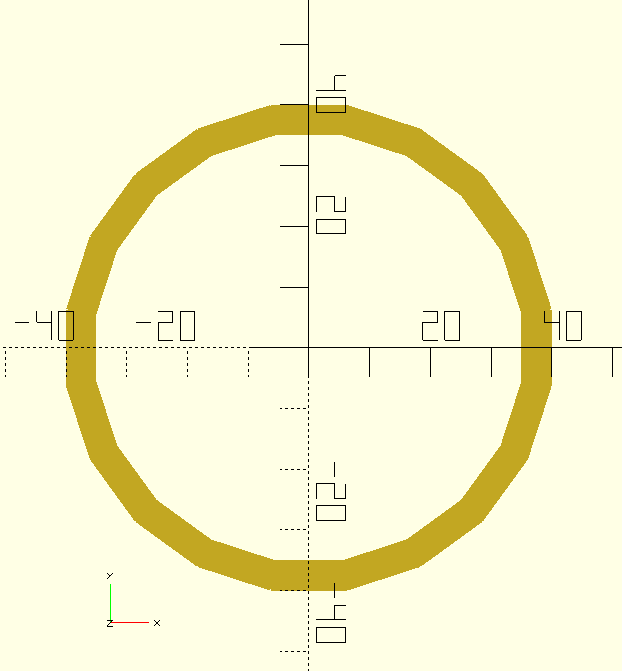
\includegraphics[width=0.48\textwidth]{imagenes/piso-solucion-1}}%
  \hfill%
  \subbottom[...ya que, contrariamente a lo deseable, los ladrillos no
  presentan intersticios entre sí.]
  {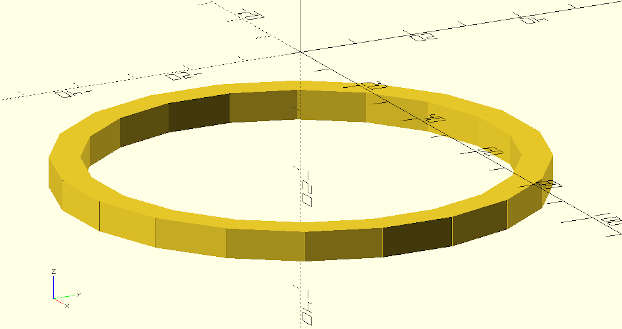
\includegraphics[width=0.48\textwidth]{imagenes/piso-sin-intersticios}}
          
        % \label{fig:piso-sin-intersticios}
        \caption{Cecilia casi soluciona el \emph{bug} de su piso.}
      \label{fig:piso-solucion-1}        
    \end{figure}




---¡Oh..! ---el entusiasmo de Cecilia se enfrió de golpe frente a la
figura \ref{fig:piso-solucion-1}: si bien el piso adquirió el radio
deseado, habían desaparecido esos bonitos intersticios que le darían
una apariencia tan característica y satisfactoria a su torre una vez
terminada.
  



---Los ladrillos están tocándose unos con otros ---re\-co\-no\-ció Cecilia
apesadumbrada.

---¡Maldita exactitud de la geometría! ---masculló Antonia, con aire
burlón, y pretendiendo darle así una pista del problema que ahora
aparecía.

Cecilia, tras unos instantes, replicó:

---Sí, entiendo: el largo de los ladrillos fue calculado precisamente
para que llene el perímetro del piso. Así que necesito que sean un
poco más chicos. No sé; a ver si modifico el cálculo de la variable
\texttt{largo} en la línea 7, multiplicándolo por un número menor que
1...

  Cecilia probó varios valores, hasta que encontró uno que le gustó:

    \begin{lstlisting}
module piso(
 radio,
 altura,
 espesor,
 n_ladrillos) {
  i_alfa=360/n_ladrillos;
  largo=2*PI*radio/n_ladrillos*0.95; 
  for (alfa=[0:i_alfa:359])
   rotate([0,0,alfa])
    translate([radio-espesor/2,0,0])
     ladrillo([espesor,largo,altura]); 
}

piso(40,5,5,20);
    \end{lstlisting}


    \begin{figure}[ht]
      \centering
      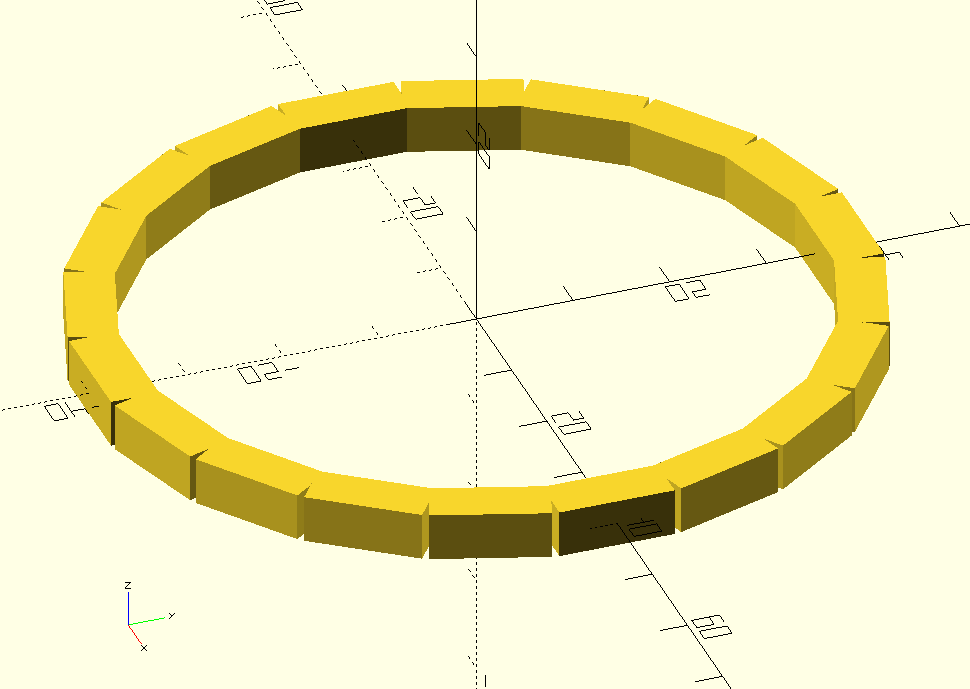
\includegraphics[width=.7\textwidth]{imagenes/piso-solucion-2}      
      \caption{Los ladrillos, ahora, se presentan con intersticios
        visualmente gratos.}
      \label{fig:piso-solucion-2}
    \end{figure}


  \section{Parámetros opcionales}

  Cecilia, feliz por el resultado conquistado, giró para mirar a
  Antonia, a tiempo de advertir que un relámpago cruzaba por los ojos
  de su amiga. <<¡Ups!>> ---pensó Cecilia--- <<¿Qué se le habrá
  ocurrido ahora?>>.

  ---Cecilia ---empezó Antonia con un tono que presagiaba más
  trabajo---; ¿estás segura de que los lectores de tu texto (entre los
  que te contarás vos misma más adelante) estarán de acuerdo con el
  valor 0,95? ¿No te parece que si tienen derecho a elegir el radio,
  espesor, altura, etc., de la torre de sus sueños, no deberían
  también poder decidir la magnitud de los intesticios entre los
  ladrillos? ---pre\-gun\-tó, con aire de no admitir otra respuesta
  que un rotundo ``Sí''.

  ---Tenés razón ---Cecilia no pudo menos que ad\-mi\-tir\-lo---; pero
  la hacemos fácil: agregamos un parámetro más al módulo:
  \lstinline!factor_inter!, y listo:

    \begin{lstlisting}
module piso(
 radio,
 altura,
 espesor,
 n_ladrillos,
 factor_inter) {
  i_alfa=360/n_ladrillos;
  largo=2*PI*radio/n_ladrillos*factor_inter; 
  for (alfa=[0:i_alfa:359])
   rotate([0,0,alfa])
    translate([radio-espesor/2,0,0])
     ladrillo([espesor,largo,altura]); 
}
    \end{lstlisting}

    ---No está mal ---aprobó Antonia displicentemente---; pero se
    puede hacer mejor. Si bien estamos de acuerdo en que es deseable
    que el lector pueda elegir, a la hora de crear un piso, la
    magnitud de los intersticios, también es cómodo ofrecerle un valor
    `convencional' y que `funciona', en caso de que no quiera ponerse
    a buscar uno por sí mismo. Para eso resultan insustituibles los
    parámetros opcionales: parámetros que, si el usuario no los
    indica, toman un valor predeterminado; mirá cómo modifico la línea
    6 ---dijo Antonia, tomando a su cargo el teclado.

    \begin{lstlisting}
module piso(
 radio,
 altura,
 espesor,
 n_ladrillos,
 factor_inter=0.95) {
  i_alfa=360/n_ladrillos;
  largo=2*PI*radio/n_ladrillos*factor_inter; 
  for (alfa=[0:i_alfa:359])
   rotate([0,0,alfa])
    translate([radio-espesor/2,0,0])
     ladrillo([espesor,largo,altura]); 
}
    \end{lstlisting}

\guillemotright Ahora, si el usuario escribe \lstinline!piso(40,5,5,20)!
  obtendrá un piso con ladrillos un 95\% (el valor `por defecto') más
  pequeños; pero si escribe \lstinline!piso(40,5,5,20,0.7)!, los ladrillos
  serán un 70\% más chicos:


  \begin{minipage}[]{.45\textwidth}
    \begin{lstlisting}[numbers=none]
  piso(40,5,5,20);
    \end{lstlisting}
  \end{minipage}\hfill
  \begin{minipage}[]{.55\textwidth}
      \centering
      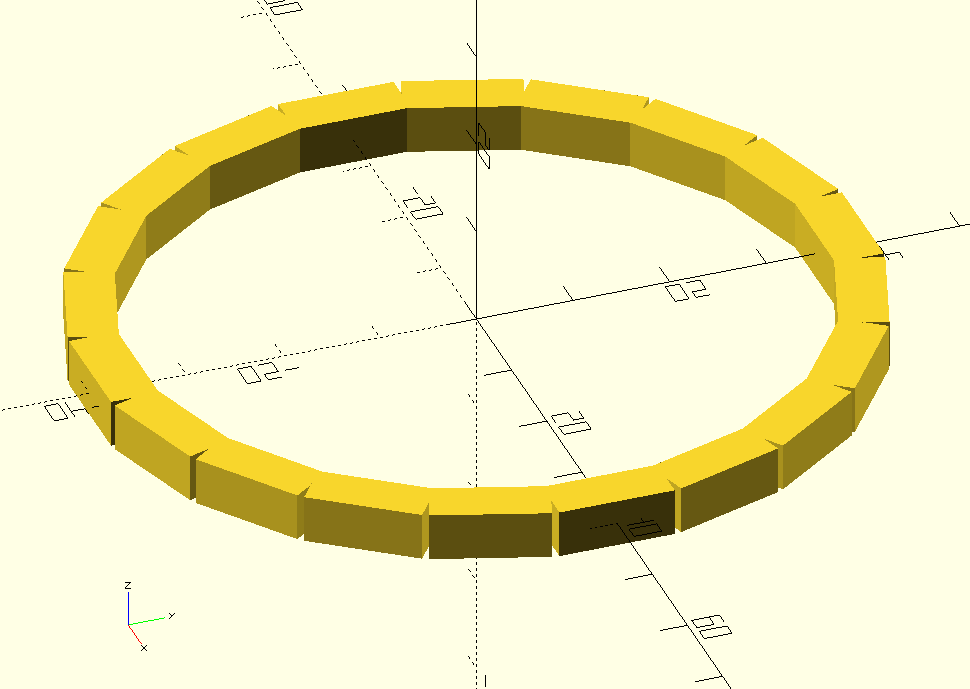
\includegraphics[width=.9\textwidth]{imagenes/piso-solucion-2}
    \end{minipage}



  \begin{minipage}[]{.45\textwidth}
    \begin{lstlisting}[numbers=none]
  piso(40,5,5,20,0.7);
    \end{lstlisting}
  \end{minipage}\hfill
  \begin{minipage}[]{.55\textwidth}
      \centering
      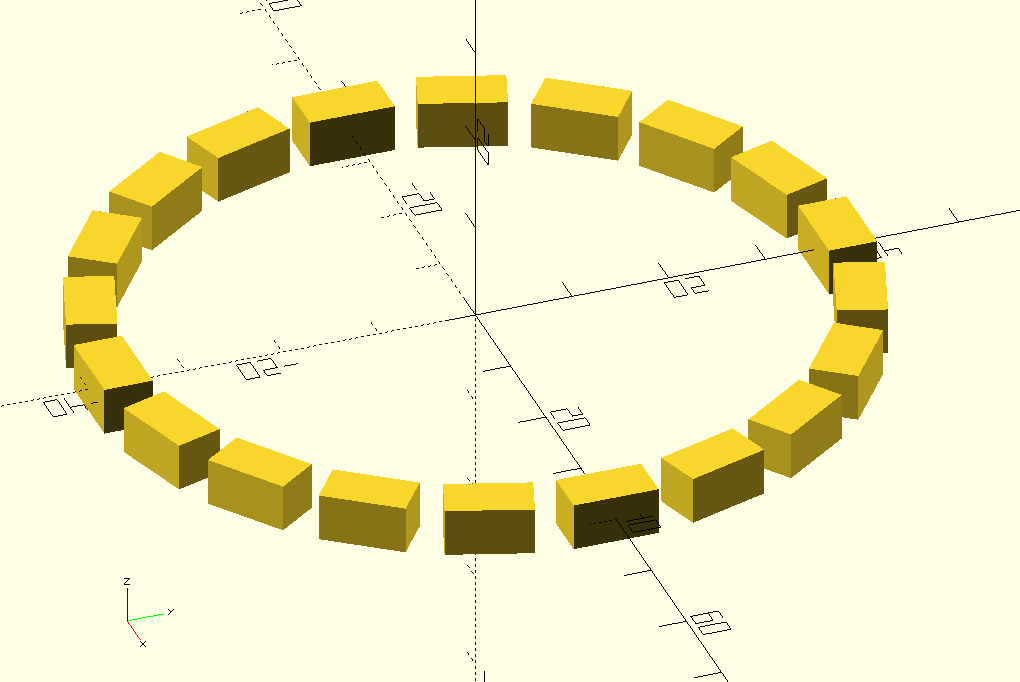
\includegraphics[width=.9\textwidth]{imagenes/piso-solucion-0-7}
    \end{minipage}

    \vspace{1em}

  Definitivamente, 0,7 era un valor muy bajo para los intersticios;
  pero Cecilia captó la idea y apreció las posibilidades que podían
  brindarle los parámetros opcionales.
  

%%% Local Variables:
%%% mode: latex
%%% TeX-master: "../libro"
%%% End:
